\chapter{Plotting with Pyplot}
\label{ch:pyplot}

\section{matplotlib.pyplot}
Matplotlib and its PyPlot environment is a versatile Python plotting
library which produces publication quality figures in a variety of
hard-copy formats such as EPS, PDF, and PNG.  With PyPlot you can
generate scatter and line plots, histograms, power spectra, bar
charts, error-charts, pie charts, and many more with just a few lines
of code. For the power user, you have full control of line styles,
font properties, axes properties, and so on. For useful examples of 
astronomy plots that can be generated with PyPlot, see Leonardo 
Ubeda's astroplotlib library at \href{http://astroplotlib.stsci.edu/}
{http://astroplotlib.stsci.edu/}


\section{Create a Simple Scatter Plot}

We'll start by making a simple scatter plot, demonstrating some of 
the PyPlot options, and saving our plot in a PDF format. 

First, we need to read in some data, as we learned in Chapter~[[...]].

\begin{alltt}
\pytab from astropy.io import ascii
\pytab data_A = ascii.read('flux_vs_time_A.dat', names=['Time',  \textbackslash 
\ldots 'Flux_pcnt_diff', 'Flux_err', 'Flux_linear_fit'])
\pytab data_C = ascii.read('flux_vs_time_C.dat', names=['Time',  \textbackslash 
\ldots 'Flux_pcnt_diff', 'Flux_err', 'Flux_linear_fit'])
\end{alltt}

The time is in Modified Julian Date (MJD) and the remaining 
columns are flux percent differences and are dimensionless. 
(The fluxes are of a standard white dwarf for a WFC3 monitoring 
program. The two datasets are from different amplifiers
on the WFC3 two-chip mosaic.)

Now we will import PyPlot and make our first plot, 
using a \textit{figure} object...

\begin{alltt}
\pytab import matplotlib.pyplot as pyplot
\pytab figure, ax = pyplot.subplots()
\end{alltt}

Now we can begin to plot into the \textit{figure} object, via the \textit{ax} 
axis created in the previous step. Each subsequent call to the inherited 
\textit{ax.plot} method will update the overall plot. The next two calls
plot the two sets of flux differences as scatter plots in blue and red,
respectively.

\begin{alltt}
\pytab ax.scatter(data_A['Time'], data_A['Flux_pcnt_diff'], c='blue')
\pytab ax.scatter(data_C['Time'], data_C['Flux_pcnt_diff'], c='red')
\pytab figure.show()
\end{alltt}

The \textit{figure.show()} command displays our changes onto the \textit{figure}
object.

We should add axis labels...

\begin{alltt}
\pytab ax.set_xlabel('Time [MJD]', fontsize=20)
\pytab ax.set_ylabel('Flux Diff [%]',  fontsize=20)
\pytab figure.show()
\end{alltt}

Finally let's save the figure. We can save as a PDF, PNG, TIFF, and
other file types; we need only to type the appropriate extension.

\begin{alltt}
\pytab figure.savefig('flux_vs_time_1.pdf')
\end{alltt}


%%%%%%%%%%%%%%%%
\begin{figure}[tbp]
  \centering
    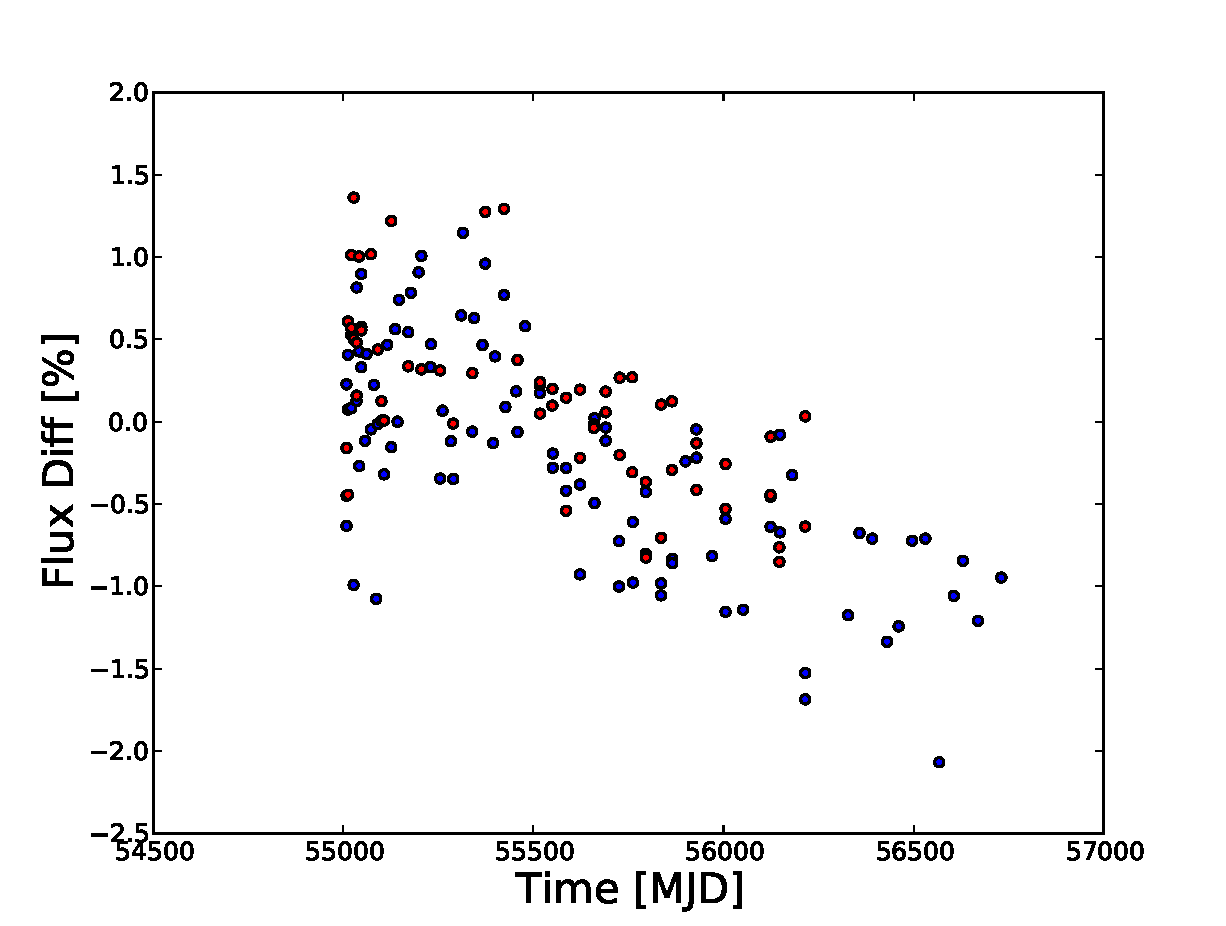
\includegraphics[scale=0.55]{flux_vs_time_1.pdf}
    \caption{Our first plot.}
  \label{fig:splot}
\end{figure}
%%%%%%%%%%%%%%%%

\section{Markers, Lines, and Legends}  %Plot customizations

We have a plot! But we are not yet finished.
PyPlot has many, many options available for you to customize
your plot. We'll demonstrate just a few for markers, lines, and legends. 

We can play with the marker type (\textit{marker}), size (\textit{s}), and 
transparency (\textit{alpha}) of our of scatter plots' points. We first
need to clear the figure with the \textit{ax.clear()} command.

\begin{alltt}
\pytab ax.clear()
\pytab ax.scatter(data_A['Time'], data_A['Flux_pcnt_diff'], \textbackslash 
\ldots   c='blue', marker='x', s=30, alpha=0.75)
\pytab ax.scatter(data_C['Time'], data_C['Flux_pcnt_diff'], \textbackslash 
\ldots   c='red', marker='d', s=30, alpha=0.75)
\pytab ax.set_xlabel('Time [MJD]', fontsize=20)
\pytab ax.set_ylabel('Flux Diff [%]', fontsize=20)
\pytab figure.show()
\end{alltt}

The plot would be clearer if we added a legend.

\begin{alltt}
\pytab ax.clear()
\pytab ax.scatter(data_A['Time'], data_A['Flux_pcnt_diff'], \textbackslash 
\ldots   c='blue', marker='x', s=25, alpha=0.75, label='Amp A')
\pytab ax.scatter(data_C['Time'], data_C['Flux_pcnt_diff'], \textbackslash 
\ldots   c='red', marker='d', s=25, alpha=0.75, label='Amp C')
\pytab ax.set_xlabel('Time [MJD]', fontsize=20)
\pytab ax.set_ylabel('Flux Diff [%]', fontsize=20)
\pytab ax.legend(loc='best', scatterpoints=1)
\pytab figure.show()
\end{alltt}

The \textit{ax.legend(loc='best')} command will try to find the least busy section 
of your plot and stick the legend there. 

Next let's plot lines with the linear fits from our data:

\begin{alltt}
\pytab ax.plot(data_A['Time'], data_A['Flux_linear_fit'], \textbackslash 
\ldots  c='blue', ls='--', linewidth=2, label='Amp A Fit')
\pytab ax.plot(data_C['Time'], data_C['Flux_linear_fit'], \textbackslash 
\ldots  c='red', ls=':', linewidth=2, label='Amp C Fit')
\pytab ax.legend(loc='best', scatterpoints=1)
\pytab figure.show()
\end{alltt}

Suppose we want to denote the 0.0 flux difference with a dashed line and the
MJD date 56250.0 with a green line:

\begin{alltt}
\pytab ax.axhline(0.0, color='k', ls='--', linewidth=1)  
\pytab ax.axvline(56250.0, color='green', ls='-', linewidth=2) 
\pytab figure.show()
\end{alltt}

%%%%%%%%%%%%%%%%
\begin{figure}[tbp]
  \centering
    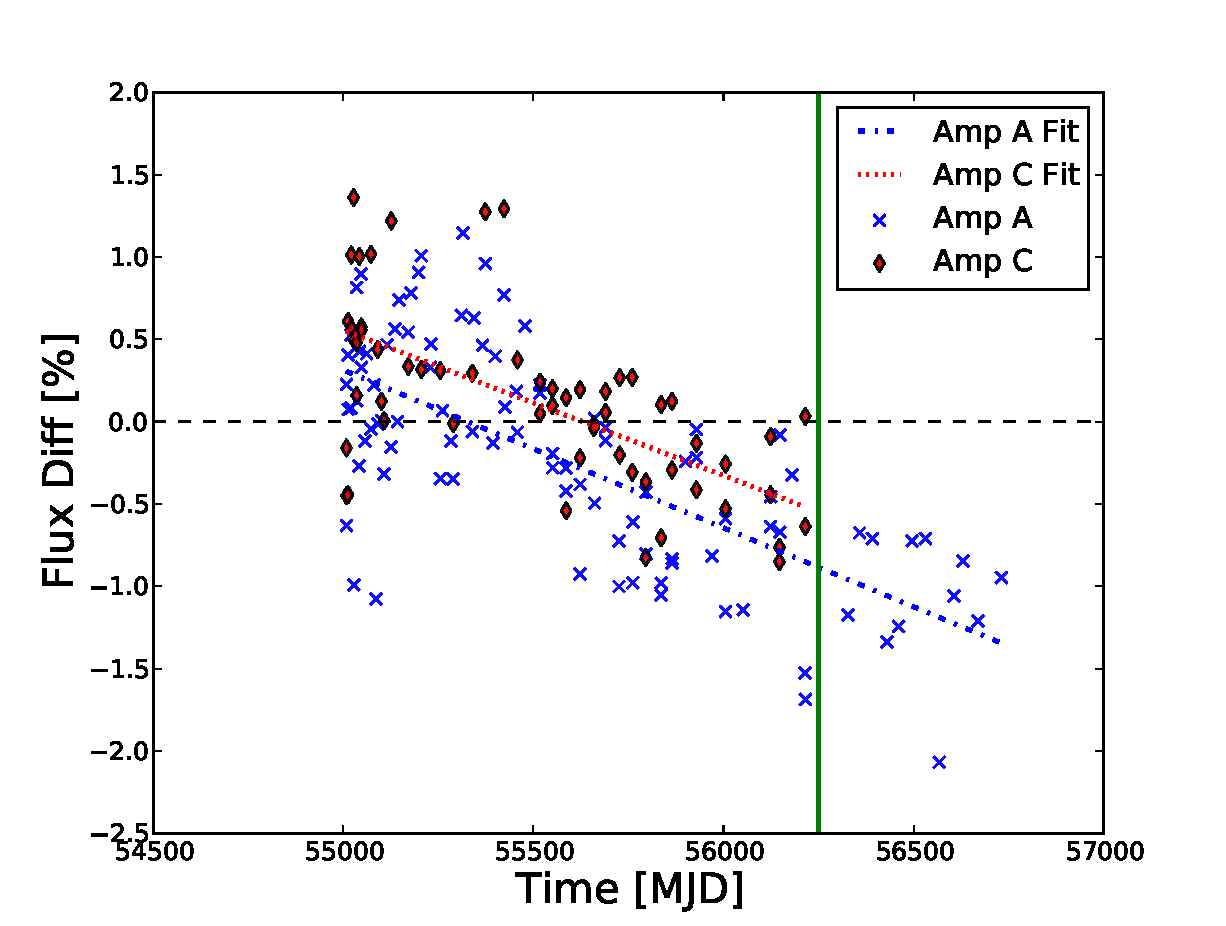
\includegraphics[scale=0.55]{flux_vs_time_2.pdf}
    \caption{Our customized plot.}
  \label{fig:splot}
\end{figure}
%%%%%%%%%%%%%%%%

We now have a personalized plot! (It doesn't have to be pretty.) Let's save it.

\begin{alltt}
\pytab figure.savefig('flux_vs_time_2.pdf')
\end{alltt}

Other options can be found on the Matplotlib PyPlot site listed in Chapter~\ref{ch:links}. 

For different color names, see \href{http://www.w3schools.com/html/html_colornames.asp}
{http://www.w3schools.com/html/html\_colornames.asp}

%http://matplotlib.org/1.2.1/examples/pylab_examples/show_colormaps.html


\section{Error Bars}

We have columns giving our error. We can display them on our plot as
error bars using the \textit{errorbar} function:

\begin{alltt}
\pytab ax.clear()
\pytab ax.scatter(data_A['Time'], data_A['Flux_pcnt_diff'], c='blue')
\pytab ax.errorbar(data_A['Time'], data_A['Flux_pcnt_diff'], \textbackslash 
\ldots yerr=data_A['Flux_err'], c='grey', marker=None, ls='None')
\pytab figure.show()
\end{alltt}


\section{Display Dates on X-axis}

MJD is a convenient format for plotting time. But who 
thinks in MJD? Let's convert MJD to day-month-year and display them 
on the x-axis. In python this is a little tricky.

\begin{alltt}
\pytab from astropy.time import Time
\pytab time_MJD = [float(item.get_text()) for item in ax.get_xticklabels()]
\pytab time_convert = Time(time_MJD, format='mjd', scale='utc')
\pytab time_ymd_long = time_convert.iso
\pytab time_ymd_short = []
\pytab for date in time_ymd_long:
\ldots    time_ymd_short.append(date.split(' ')[0])
\pytab ax.set_xticklabels(time_ymd_short)
\pytab figure.show()
\end{alltt}


See \href{http://astropy.readthedocs.org/en/latest/time/}{http://astropy.readthedocs.org/en/latest/time/} for more examples.



\section{Plot Figures Side-by-Side}

%many examples from ...


\section{Fitting Lines}



\section{Display a FITS Image}
%Different examples of drawing over image.


\section{Plot Spectra}








\section{Plot with Pyplot}
From Section~\ref{ss:loadtxt} we learned how to read in data from a
file, particularly Gordon2005\_Fig16.txt.  We will reproduce the slope
plot in Figure~16 of the Gordon 2005 paper.

\begin{alltt}
\pytab import numpy as np 
\pytab infile = 'Gordon2005_Fig16.txt' 
\pytab slope, ran_slope_unc, corr_slope_unc, \textbackslash 
\ldots      both_slope_unc, eqn_slope_unc = np.loadtxt(infile, 
\ldots      usecols=(0, 1, 2, 3, 4), unpack=True) 
\end{alltt}

These arrays have nice descriptive names, but to help make the
plotting process clear, we will assign short names.

\begin{alltt}
\pytab xx = slope  
\pytab yy1 = ran_slope_unc  
\pytab yy2 = corr_slope_unc  
\pytab yy3 = both_slope_unc
\pytab yy4 = eqn_slope_unc 
\end{alltt}

Now we will import Pyplot and make our first plot, using a \textit{figure} 
object...

\begin{alltt}
\pytab import matplotlib.pyplot as plt  
\pytab figure, ax = plt.subplots()
\end{alltt}

Now we can begin to plot into the \textit{figure} object, via the \textit{ax} 
axis created in the previous step. Each subsequent call to the inherited 
\textit{ax.plot} method will update the overall plot... 

\begin{alltt}
\pytab ax.plot(xx, yy1, ls='--', color='b')
\pytab ax.plot(xx, yy2, ls=':', color='r')
\pytab ax.plot(xx, yy3, ls='-', color='g')
\pytab ax.plot(xx, yy4, ls='-.', color='m')
\end{alltt}

Notice that `b' is for blue, `r' is for red, `g' is for green, and `m'
is for magenta.  Furthermore, `-' is for a solid line, `--' is for a
dashed line, `:' is for a dotted line, and `-.' is for a dot-dash
line.  Several other options are available as well and can be found on
the Matplotlib Pyplot site listed in Chapter~\ref{ch:links}. 

The lines are pretty faint, and we also need to add a legend and axis
labels. Let's start by clearing the \textit{axis} object, replotting, and then 
force a refresh on our \textit{figure}:

\begin{alltt}
\pytab ax.clear()
\pytab ax.set_xlabel('Slope [e-/s]')
\pytab ax.set_ylabel('Slope Uncertainty [e-/s]')
\pytab ax.plot(xx, yy1, ls='--', color='b', label='Randon Unc.')
\pytab ax.plot(xx, yy2, ls=':', color='r', label='Correlated Unc.')
\pytab ax.plot(xx, yy3, ls='-', color='g', label='Both')
\pytab ax.plot(xx, yy4, ls='-.', color='m', label='Equation')
\pytab ax.legend(loc='best')
\pytab figure.show()
\end{alltt}

We can save this plot.  The figure will save as a PDF, PNG, TIFF, and
others depending on the name given.

\begin{alltt}
\pytab figure.savefig('fig16.pdf')
\pytab figure.clf()
\end{alltt}

Notice that we cleared the figure with \textit{figure.clr()}. This step is not 
necessary, but is useful to clear a figure object that is no longer needed. 
Open fig16.pdf and take a look.  It looks pretty good, right?

\begin{figure}[tbp]
  \centering
    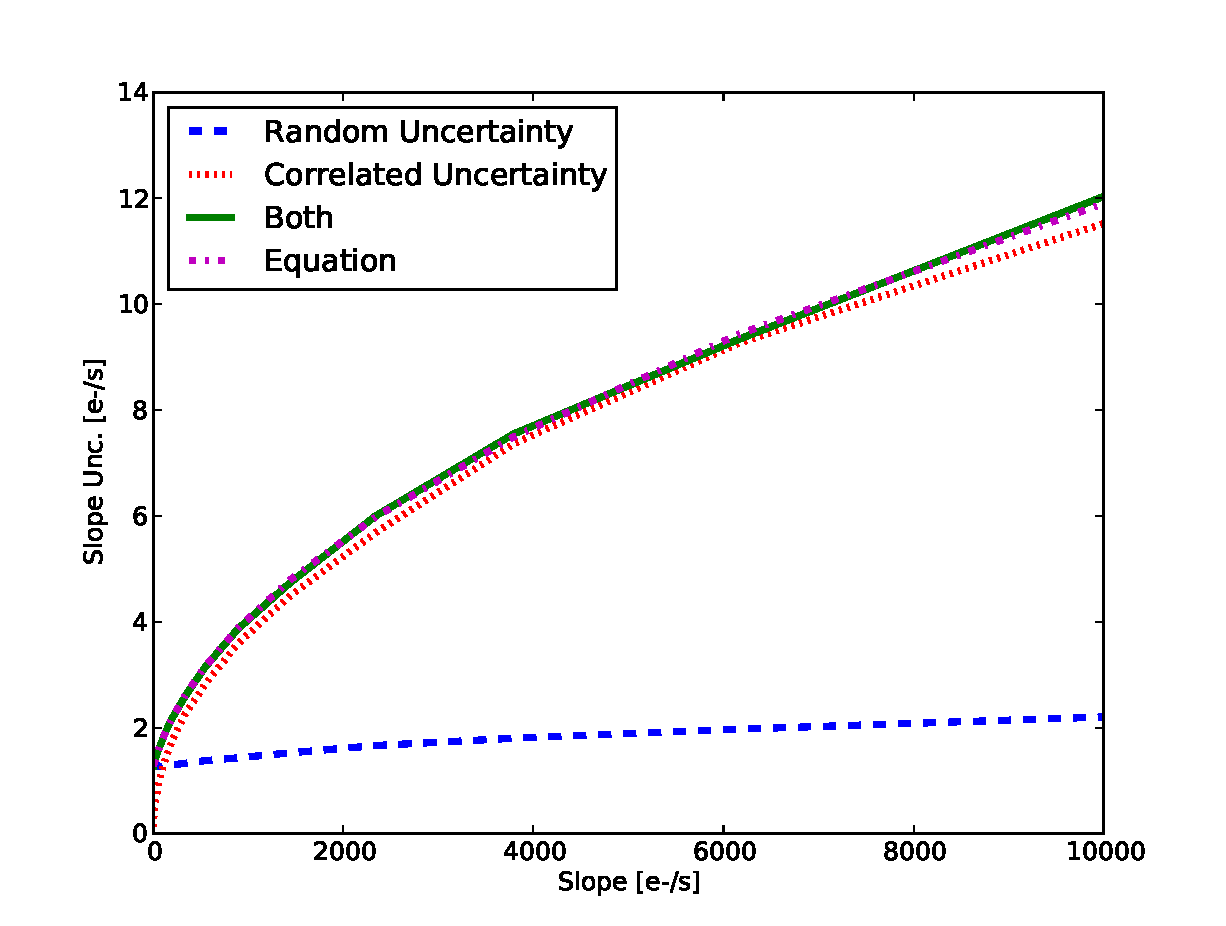
\includegraphics[scale=0.55]{splot.pdf}
    \caption{Our first try at re-creating Figure 16 in Gordon 2005.}
  \label{fig:splot}
\end{figure}

If you look at the paper by
Gordon et al. 2005, though, you will see that the key thing we are missing is
logarithmic axis.  Instead of \textit{matplotlib.pyplot.plot} we will use \textit{matplotlib.pyplot.loglog}:

\begin{alltt}
\pytab ax.clear()      # Clear the axis...
\pytab ax.loglog(xx, yy1, ls='--', lw=3, color='b', label='Random Unc.')
\pytab ax.loglog(xx, yy2, ls=':', lw=3, color='r', label='Correlated Unc.')
\pytab ax.loglog(xx, yy3, ls='-', lw=3, color='g', label='Both')
\pytab ax.loglog(xx, yy4, ls='-.', lw=3, color='m', label='Equation')

\pytab ax.set_xlabel('Slope [e-/s]')
\pytab ax.set_ylabel('Slope Uncertainty [e-/s]')
\pytab ax.legend(loc='best')
\pytab figure.show()
\end{alltt}

Again, open the figure you just made.  How does that look?  

\begin{figure}[tbp]
  \centering
    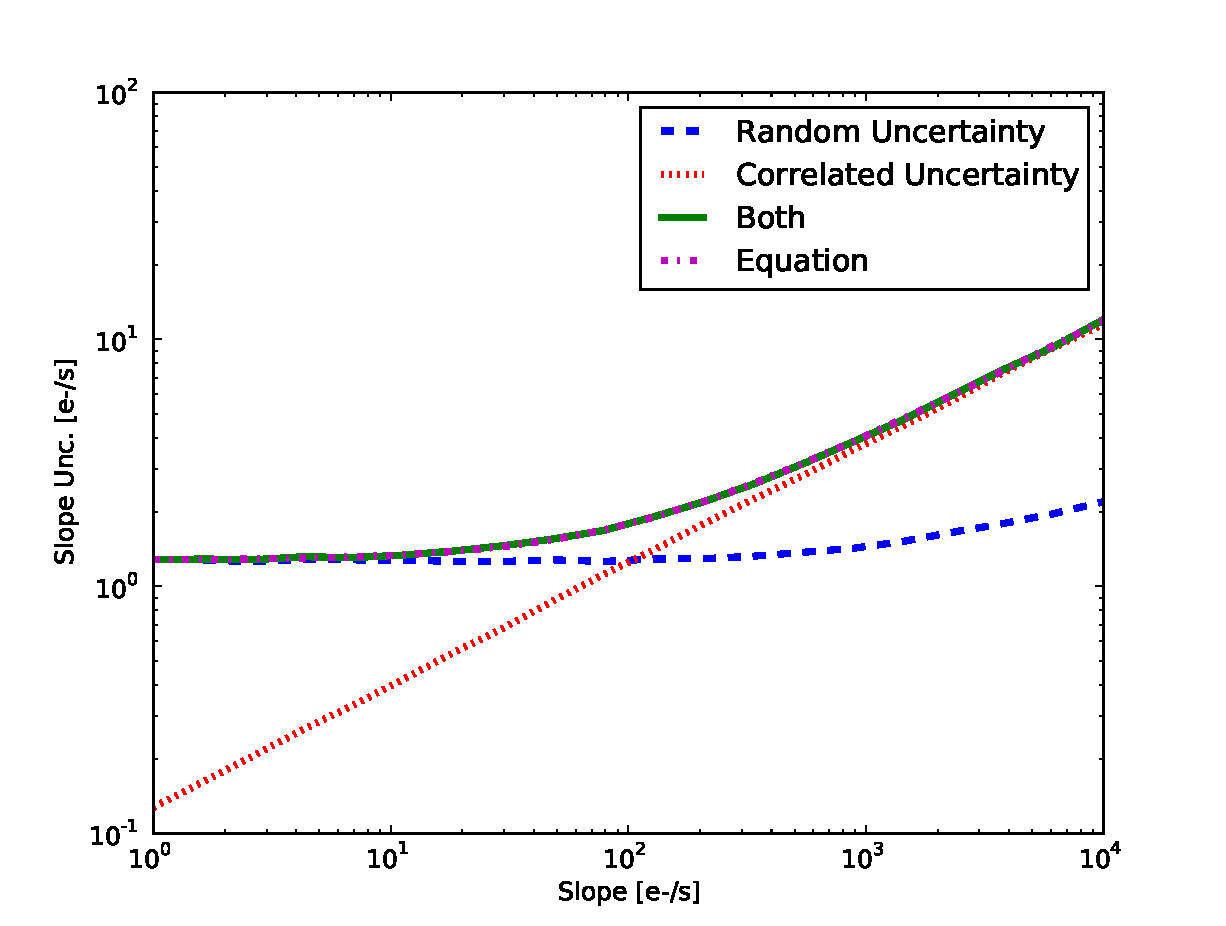
\includegraphics[scale=0.6]{splot_log.pdf}
    \caption{Our version of Figure 16 in Gordon 2005.}
  \label{fig:splot}
\end{figure}

For more
plotting options with Matplotlib and Pyplot, check out the 
\href{http://matplotlib.org/}{matplotlib.org} link listed in
Chapter~\ref{ch:links}.  Notice that there is a link to NumPy on this
page, as well as links to screen-shots, thumbnails, and examples.

Our plot is looking good, however this is getting way too messy.
Isn't there a way we can keep this all nicely in a file, where we can
type it once correctly and never have to type it again?  Sure there
is!  We need to write a script.
